\section{Simulation Results}
			\label{sec:simul}
%%%In this section, we report a summary of simulation experiments to evaluate the performance of the proposed algorithms. 
			
			
						\begin{figure*}[t]	
				\centering
				\begin{subfigure}[b]{0.25\textwidth}
					\begin{center}
						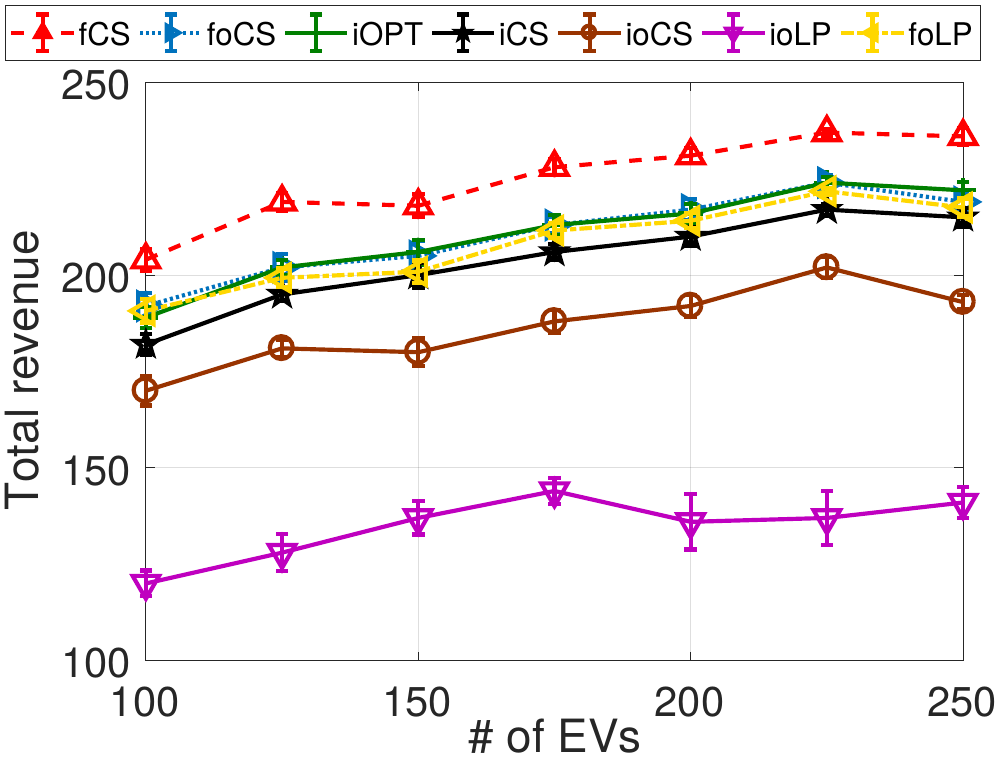
\includegraphics[width=\textwidth]{V-N-M2.png}
						\caption{\revv{$m=2$}}
						\label{fig:V-N-M2}
					\end{center}
				\end{subfigure}
				\begin{subfigure}[b]{0.25\textwidth}
					\begin{center}
						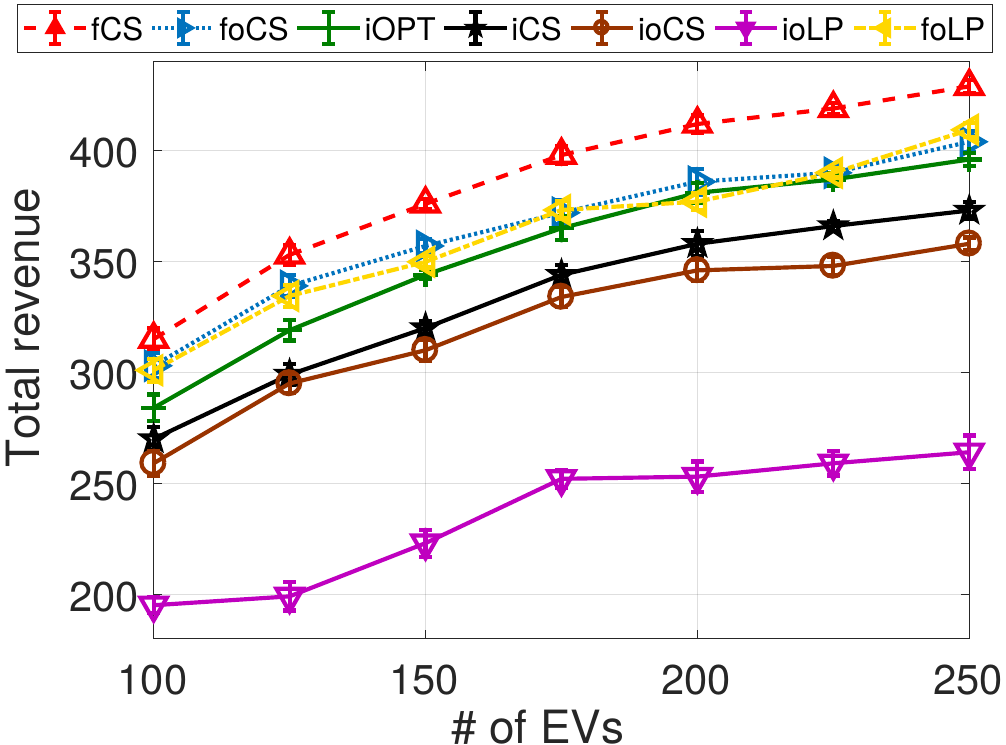
\includegraphics[width=\textwidth]{V-N-M4.png}
						\caption{\revv{$m=4$}}
						\label{fig:V-N-M4}
					\end{center}
				\end{subfigure}% 	
				\begin{subfigure}[b]{0.25\textwidth}
					\begin{center}
						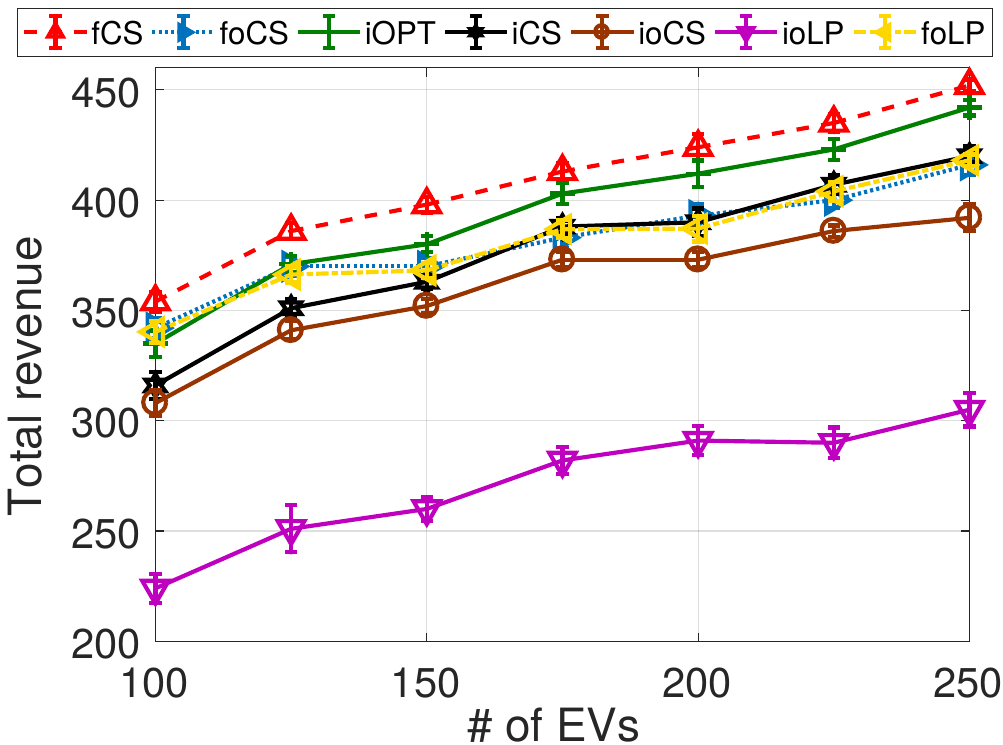
\includegraphics[width=\textwidth]{V-N-M8.png}
						\caption{\revv{$m=8$}}
						\label{fig:V-N-M8}
					\end{center}
				\end{subfigure}% 
				\caption{Comparison results for $2$, $4$, and $8$ CSs for fractional and integral revenue models. In the algorithms' name, letters ``o'', ``f'' and ``i'' indicate online, fractional and integral, respectively. Note that a ``non-optimal'' fractional algorithm can potentially achieve better result than an ``optimal'' integral algorithm due to higher flexibility in power allocation.}  
				\label{fig:V-N-M}
%				\vspace{-3mm}
			\end{figure*}
%\subsection{Simulation Setup and Overview}
\textit{Simulation Setup and Overview:} We consider charging scheduling of EVs \revv{during a period of $12$ time slots of length $1$ hour (e.g., from $08$:$00$ to $20$:$00$)}. 
We gathered information of \revv{$12$} popular EV models in the market to use in the simulation. Each EV model is characterized by its battery capacity as shown in Table \ref{tb:models} and maximum charging rate. \revv{Tesla models can get charged with up to $100$ kW using Tesla super chargers. Also, all other models have rapid DC charging capability (up to $50$ kW) with CHAdeMO method. This setting for charging rates is in accordance with future DCFC systems that can have several fast DC chargers installed in the charging station.} 
%Battery capacity varies from \revv{$14$} kWh to \revv{$100$} kWh and the maximum charging rate from \revv{$3.3$} kW to \revv{$22$} kW. 
%As in \cite{Tang,Chen}, we assume that arrival times follow a Poisson distribution and parking times follow an exponential distribution.
% with the mean arrival and parking duration indicated in Table \ref{tb:a-d}. 
The peak intervals include $08$:$00$-$10$:$00$, $12$:$00$-$14$:$00$, and $18$:$00$-$20$:$00$ according to NHTS survey~\cite{Santos, Tang}. \revv{The probability of an EV's arrival during the peak hours is two times higher than the off-peak periods.
			Demands are uniform random values from 
			$[\frac{1}{2}U_i,U_i]$} where $U_i$ is the battery capacity for EV $i$ in Table~\ref{tb:models}. \revv{The deadline of each EV is set according to slackness parameter $s$ (with default value of $1.2$), its demand and maximum charging rate of the battery as $d_i=a_i+\lceil \frac{D_is}{k_i} \rceil -1$.} 
%			The minimum electricity cost is $\$0.11$ per kWh based on US national electricity price average~\cite{kWhcost}. In our setting, users can submit higher prices than the minimum price in order to ensure receive their requested demand. 
			\revv{EVs are assigned to different CSs randomly and given as input to the algorithms. The willingness to pay by each user for one kWh of power is a random uniform number from interval $[\frac{1}{2} z,\frac{3}{2}z]$ where $z=\$0.11$ is national average price of electricity in the US\cite{kWhcost}.}			
			%The default value of local peak constraint is \rev{$100$} kW and the global peak constraint is \rev{$200$} kW. We investigate the effect of this parameter in~\cite{alinia2017online}. 
			In the simulation, the results are plotted with $95\%$ confidence level and each point represents average result of $50$ random scenarios. 

Table \ref{tb:comparisons} explains the comparison algorithms including current implemented algorithm in Caltech ACN referred to as \folp \cite{lee2018adaptive} and its adapted version for the integral revenue model \iolp. The \iolp and \folp algorithms run as follows: at each time slot assume that there will be no further arrivals and solve the optimization problem (e.g., by commercial solvers) for the current set of EVs and their remaining demands. In Table \ref{tb:comparisons}, the letters ``\textsc{i}'', ``\textsc{f}'' and ``\textsc{o}'' in front of the algorithms' name refer to integral, fractional and online types, respectively.
			
			The measured performance metrics are total revenue, percentage of EVs that received all their demand, and total peak. \revv{To calculate optimal solution in integral revenue model, we used Gurobi solver \cite{optimization2013gurobi}.} 
			
						
\begin{table}[!t]
				\centering
				\caption{\revv{EV models and their battery capacity.}}
				\label{tb:models}\revv{
				\begin{tabular}{ | l| c | l| c |}
					\hline
					\textbf{Model} & \textbf{Battery} & \textbf{Model} & \textbf{Battery} \\ \hline\hline    
				Mitsubishi i-MiEV & $16$ kWh & Citroen C-Zero & $14$ kWh \\ \hline
				Peugeot iOn  & $16$ kWh & Honda Clarity & $25.5$ kWh\\\hline
				Hyundai Kona & $64$ kWh & Nissan LEAF & $40$ kWh \\ \hline
				Hyundai Ioniq & $28$ kWh & BMW i3 & $22/33$ kWh \\ \hline
				Tesla Model S/X  & $60/100$ kWh & Kia Soul EV  & $27$ kWh\\\hline
				\end{tabular}}
			\end{table}
			
%\begin{table}[h]
%				\centering
%				\caption{Arrival rates and mean parking times.}
%				\label{tb:a-d}
%				\begin{tabular}{ | l | c | c |}
%					\hline
%					\textbf{Interval} & \textbf{Arrival rate} & \textbf{Mean parking time} \\ \hline\hline    
%					$08$:$00$-$10$:$00$&  $14$&$10$\\\hline  
%					$10$:$00$-$12$:$00$&  $10$&$1/2$\\\hline 
%					$12$:$00$-$14$:$00$&  $20$&$2$\\\hline 
%					$14$:$00$-$18$:$00$&  $10$&$1/2$\\\hline
%					$18$:$00$-$20$:$00$&  $20$&$2$\\\hline
%					$20$:$00$-$24$:$00$&  $10$&$10$\\\hline
%					$24$:$00$-$08$:$00$&  $0$&$0$\\\hline
%				\end{tabular}
%\end{table}

\begin{table}[!t]
\centering
\caption{Acronyms for the algorithms}
\label{tb:comparisons}
\begin{tabular}{ | l| p{6cm}|}
\hline
\textbf{Notation} & \textbf{Description} \\ \hline\hline
\textsc{iOpt} & Optimal value under integral revenue model\\ \hline 	 
\ics & Proposed offline algorithm for \MCSP under integral revenue model\\ \hline
\fcs & Proposed \emph{optimal} algorithm for \MCSP under fractional revenue model\\\hline 
\iocs & Proposed online algorithm for \MCSP under integral revenue model\\ \hline
\focs & Proposed online algorithm for \MCSP under fractional revenue model\\ \hline
\iolp & Algorithm in \cite{lee2018adaptive} (works under integral revenue model)\\ \hline
\folp & Adaptation of algorithm in \cite{lee2018adaptive} for fractional revenue model\\ \hline
GreedyRTL & The algorithm in \cite{Jain} for single station scenario without global peak 			constraint (works under integral revenue model)\\\hline				
\end{tabular}
\end{table}
			%to simulate: Fig. 1 with M=1,4,8			
			\begin{figure*}[t!]	
				\centering
				\begin{subfigure}[b]{0.25\textwidth}
					\begin{center}
						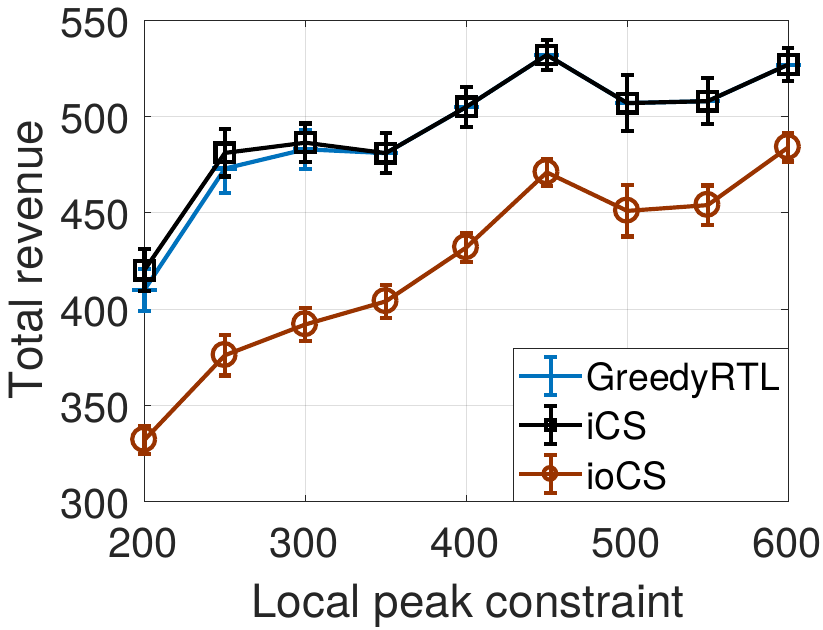
\includegraphics[width=\textwidth]{v-c.png}
						\caption{\revv{Total revenue}}
						\label{fig:v-c}
					\end{center}
				\end{subfigure}%
				%\hspace{4mm}
				\begin{subfigure}[b]{0.25\textwidth}
					\begin{center}
						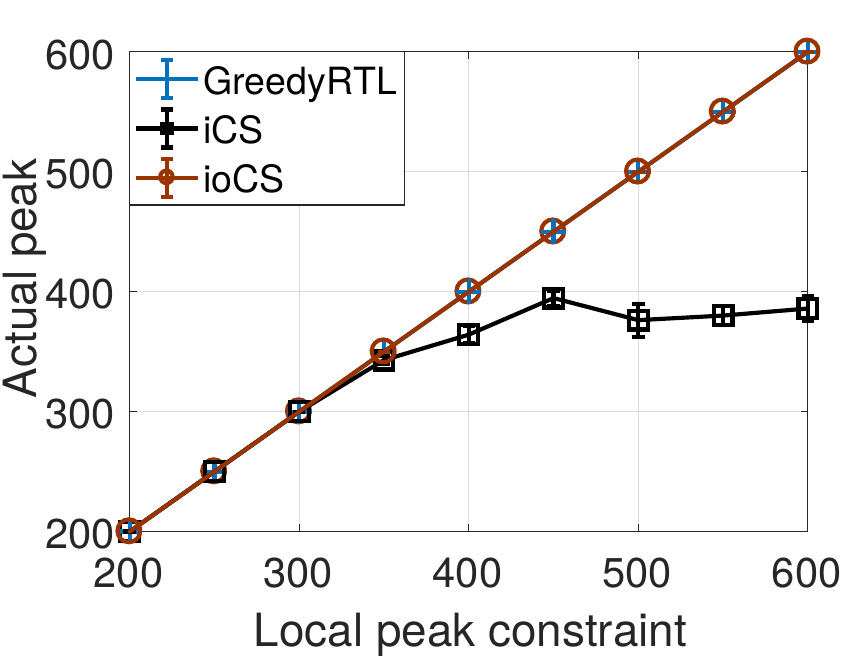
\includegraphics[width=\textwidth]{p-c.png}
						\caption{\revv{Actual global peak} 
%							($p^{\mathsf{total}}=480$)
}
						\label{fig:p-c}
					\end{center}
				\end{subfigure}%  
				%\hspace{4mm}
				\begin{subfigure}[b]{0.25\textwidth}
					\begin{center}
						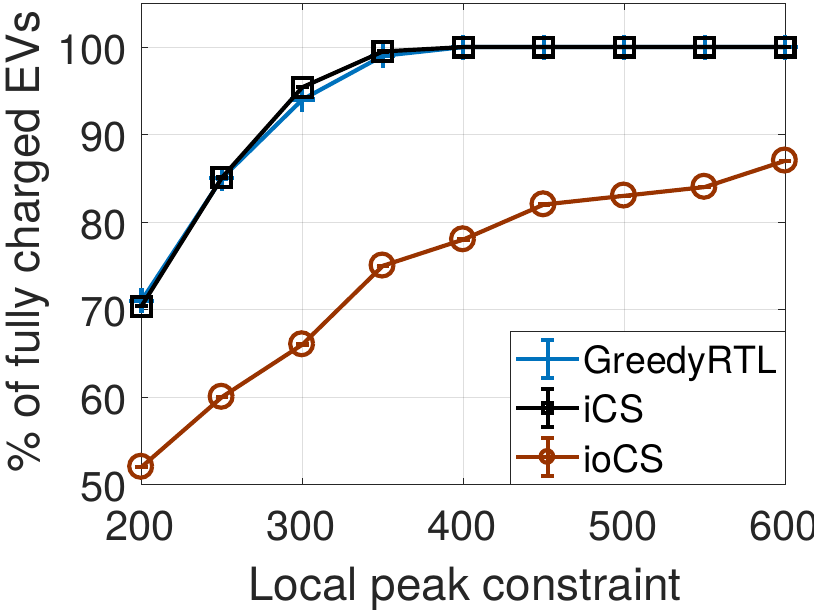
\includegraphics[width=\textwidth]{acc-c.png}
						\caption{\revv{\% of full charged EVs}}
						\label{fig:acc-c}
					\end{center}
				\end{subfigure}% 				
				\caption{\revv{Comparison in terms of total revenue, actual peak, and percentage of fully charged EVs by varying local peak value}.} 
				\label{fig:peak_local}
%			\vspace{-4mm}
			\end{figure*}
\textit{Evaluation Based on Total Revenue:}
\revv{Fig. \ref{fig:V-N-M} depicts the comparison results based on total revenue under fractional and integral models} while the total number of EVs increases from $100$ to $250$ for $2$, $4$, and $8$ CSs. \revv{The local and global peak constraints are set to $50$ kWh and $200$ kWh, respectively.}

The proposed algorithms are compared to the optimal offline solution of integral model ($\textsc{iOPT}$) and $\iolp$. Note that comparison with offline optimal could be considered as a baseline comparison with the category of approximate offline algorithms in integral model~\cite{yao2016real}.

%%% which is the running online algorithm in the Caltech ACN \cite{lee2018adaptive}. 
%The proposed algorithms for fractional revenue model, \fcs and \focs, are compared to fractional version of OLP algorithm (referred to as \folp), which is implemented in Caltech ACN  (see~\cite{alinia2017online} for details). 
Recall that \fcs is optimal offline solution. The notable observations  are  as  follows:  (i)  the  general  trend in scenario of Fig.~\ref{fig:V-N-M} is that  by increasing  the  number  of  EVs,  total  revenue  increases.  This is because with more number of EVs, the scheduler has more freedom to choose more valuable EVs. (ii)  as  explained in Section~\ref{sec:fractional}, under fractional charging model, better results are expected due to increased scheduling flexibility in CSs. According to the simulation data that we extracted from Fig.~\ref{fig:V-N-M}, the gain obtained by \fcs and \focs in Fig. \ref{fig:V-N-M} are respectively \revv{$12\%$ and $10\%$} more than the gain of the \ics and \iocs. (iii) \revv{In Fig. \ref{fig:V-N-M2} and Fig. \ref{fig:V-N-M4}, sum of the local peaks is less than or equal to the global peak while in Fig. \ref{fig:V-N-M8} this sum is two times greater than the global peak. Consequently, the total revenue significantly improved when the number of CSs is increased from $2$ to $4$ while there is a slight improvement from $4$ to $8$ CSs as the global peak constraint prevents the algorithms from charging more EVs.}
 (iv) in integral revenue model, the proposed \iocs algorithm acts significantly better than \iolp. In particular, \iocs improves \iolp by \revv{$38\%, 36\%$, and $32\%$} for $m=2$, $m=4$ and $m=8$, respectively. \revv{In fractional revenue model, however, there is a very slight difference between \focs and \folp.}
 %We highlight that \iocs (\focs) is also better choice in terms of the algorithm complexity compared to \iolp (\folp).
(v) \ics approximates \textsc{iOpt} by \revv{$97\%$, $94\%$, and $95\%$} for $m=2$, $m=4$, and $m=8$, respectively. On average, \iocs is \revv{$90\%$} of \textsc{iOpt} and, \focs is \revv{$94\%$} of its optimal offline solution, \fcs.  
(vi) finally, the results depict that \ics achieves much better results in practice as compared to the theoretical approximation ratio that characterizes the performance in worst-case scenario.

%Also, there is a sharp decline in the gap between the online methods (i.e., \focs and \iocs) and the offline solutions (i.e., \textsc{iOpt}, \ics and \fcs).


			
\revv{\emph{Comparison Based on Actual Peak:}} The constraint set in the \MCSP assures that any feasible solution respects the local and global peak constraints.
% i.e., at each time slot, the electricity consumed by station $j$ is less than or equal to $p_j$ and accumulative charging rate of all stations are less than or equal to $p^\mathsf{total}$ (note that there is no assumption that $\sum_j p_j\leq p^\mathsf{total}$, in general). 
An efficient scheduling algorithm may take a further step by not only satisfying the peak constraints but to further reduce the peak as much as possible. The proposed offline algorithms (i.e., \ics and \fcs) apply valley-filling policy to reduce the peak. The  online algorithms (i.e., \iocs and \focs) do not apply the same policy as they do not have future knowledge to be able to balance allocated resources. 
%Besides, due to uncertainties in future EV charging load in online scheduling design, it is a natural heuristic to charge EVs at earliest time.
% (i.e., setting the charging rates to the maximum feasible value at each time slot) as applied by \iocs an \focs. 
%This heuristic works well as the uncertainty in EVs' arrival time and demands may not give a second opportunity to the scheduler to charge the current EVs at the next slots. Therefore, although it is expected that \iocs and \focs have higher peak values compared to the offline algorithms, the idea of valley-filling can decrease their average response time.
% (see~\cite{alinia2017online} for the extended version of experiments).
To investigate the effect of employed valley-filling strategy, we conducted a set of simulations by varying local peak constraints. 
%from $50$ kWh to $120$ kWh and $200$ EVs. 
The results of \ics is compared to \iocs and GreedyRTL~\cite{Jain} where the latter is an approximation scheduling for single station scenario with EVs having same arrival time (see the explanations after formulating the \MCSP in Section \ref{sec:problem}). 
%The GreedyRTL algorithm works under integral revenue model. Therefore, results for \fcs and \focs are not plotted. 
%Since GreedyRTL assumes all EVs arrive at the same time, we set all arrival times to $1$. Moreover, we assume that global peak constraint is big enough (i.e., $\sum_{j=1}^m p_j\leq p^\textsf{total}$) such that the solution of GreedyRTL is feasible. We run GreedyRTL in each CS separately and combine the results. 
The results are shown in Fig.~\ref{fig:peak_local}.  
Along with total revenue in Fig.~\ref{fig:v-c}, we also report total \emph{actual} peak in Fig.~\ref{fig:p-c} and percentage of fully charged EVs in Fig.~\ref{fig:acc-c}. 
%As a high level trend, the results show that as the peak values increase, total revenue, total actual peak, and the number of EVs who received all their demand increase.  
In Fig. \ref{fig:v-c}, the results for \ics and GreedyRTL are almost identical while \iocs is \revv{$90\%$} of the other two algorithms, on average. When \revv{$p_j\geq 400$}, the total revenue for \ics and GreedyRTL does not increase in Fig. \ref{fig:v-c} and percentage of fully charged EVs is $100$ for both algorithms according to Fig. \ref{fig:acc-c}. From this point and onward, the scheduling is not challenging for offline methods to obtain optimal answer because of resource sufficiency. However, it is still a challenge to control total actual peak for the system. As a result of valley-filling policy, the value of actual peak of \ics in Fig. \ref{fig:p-c} remains almost unchanged for \revv{$p_{j}\geq 400$}.  \iocs and GreedyRTL, however, continuously increase the peak demand, since they are not using any peak shaving approach.
% and only try to maximize total revenue. 
%According to Fig. \ref{fig:p-c}, \iocs always reaches to the maximum peak of $\sum_j p_j$.
			
			
%A glance at Table \ref{tb:models} shows that in general, an EV needs a minimum time of $2$ hours to get $70\%$ of its battery capacity if charging rate is set to the maximum value. However, CSs are allowed to preempt the charging at any time and set charging rate any value lower than the maximum rate. Therefore, average response times can be higher as it can be seen in Fig. \ref{fig:rt-c}.
			
%\begin{figure}[t]	
%\centering
%				\begin{subfigure}[b]{0.25\textwidth}
%					\begin{center}
%						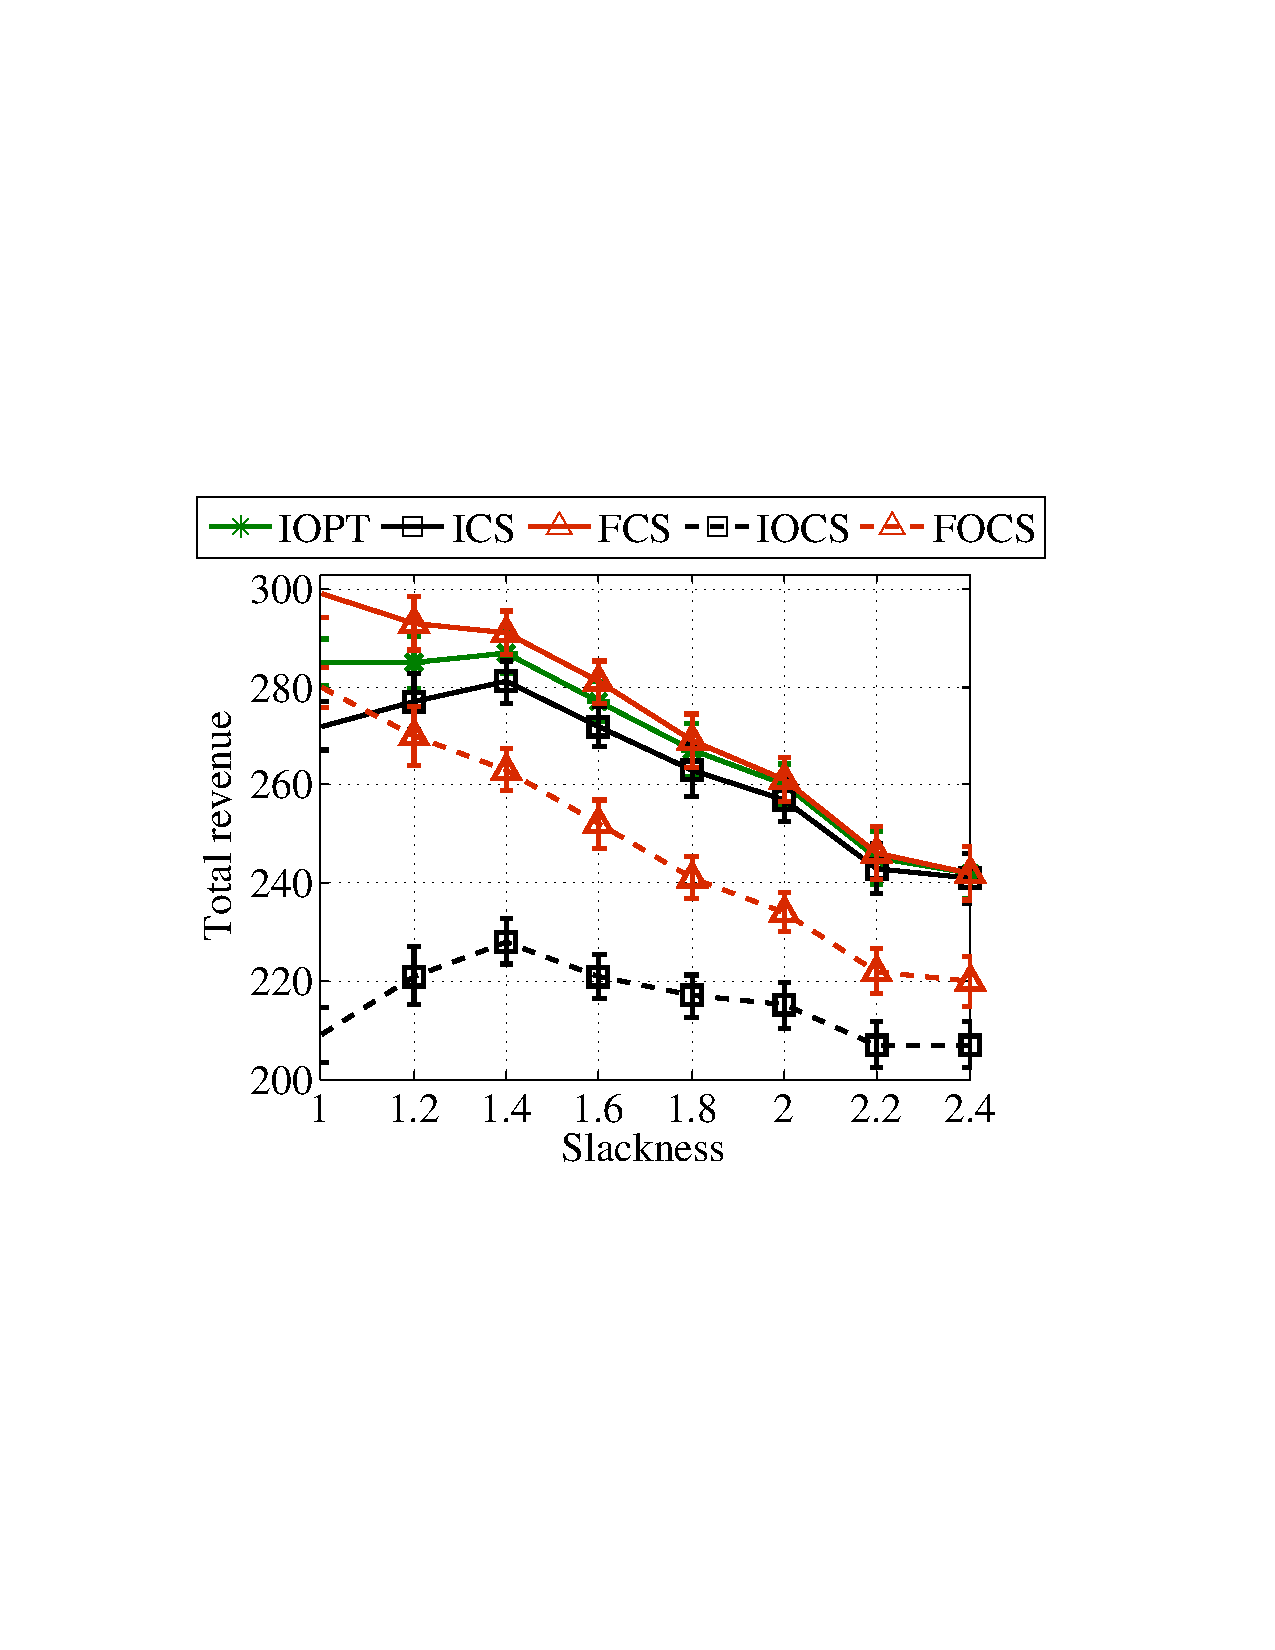
\includegraphics[width=\textwidth]{v-s-method1.pdf}
%						\caption{Total revenue (\$)}
%						\label{fig:v-s-method1}
%					\end{center}
%				\end{subfigure}%				
%				\begin{subfigure}[b]{0.25\textwidth}
%					\begin{center}
%						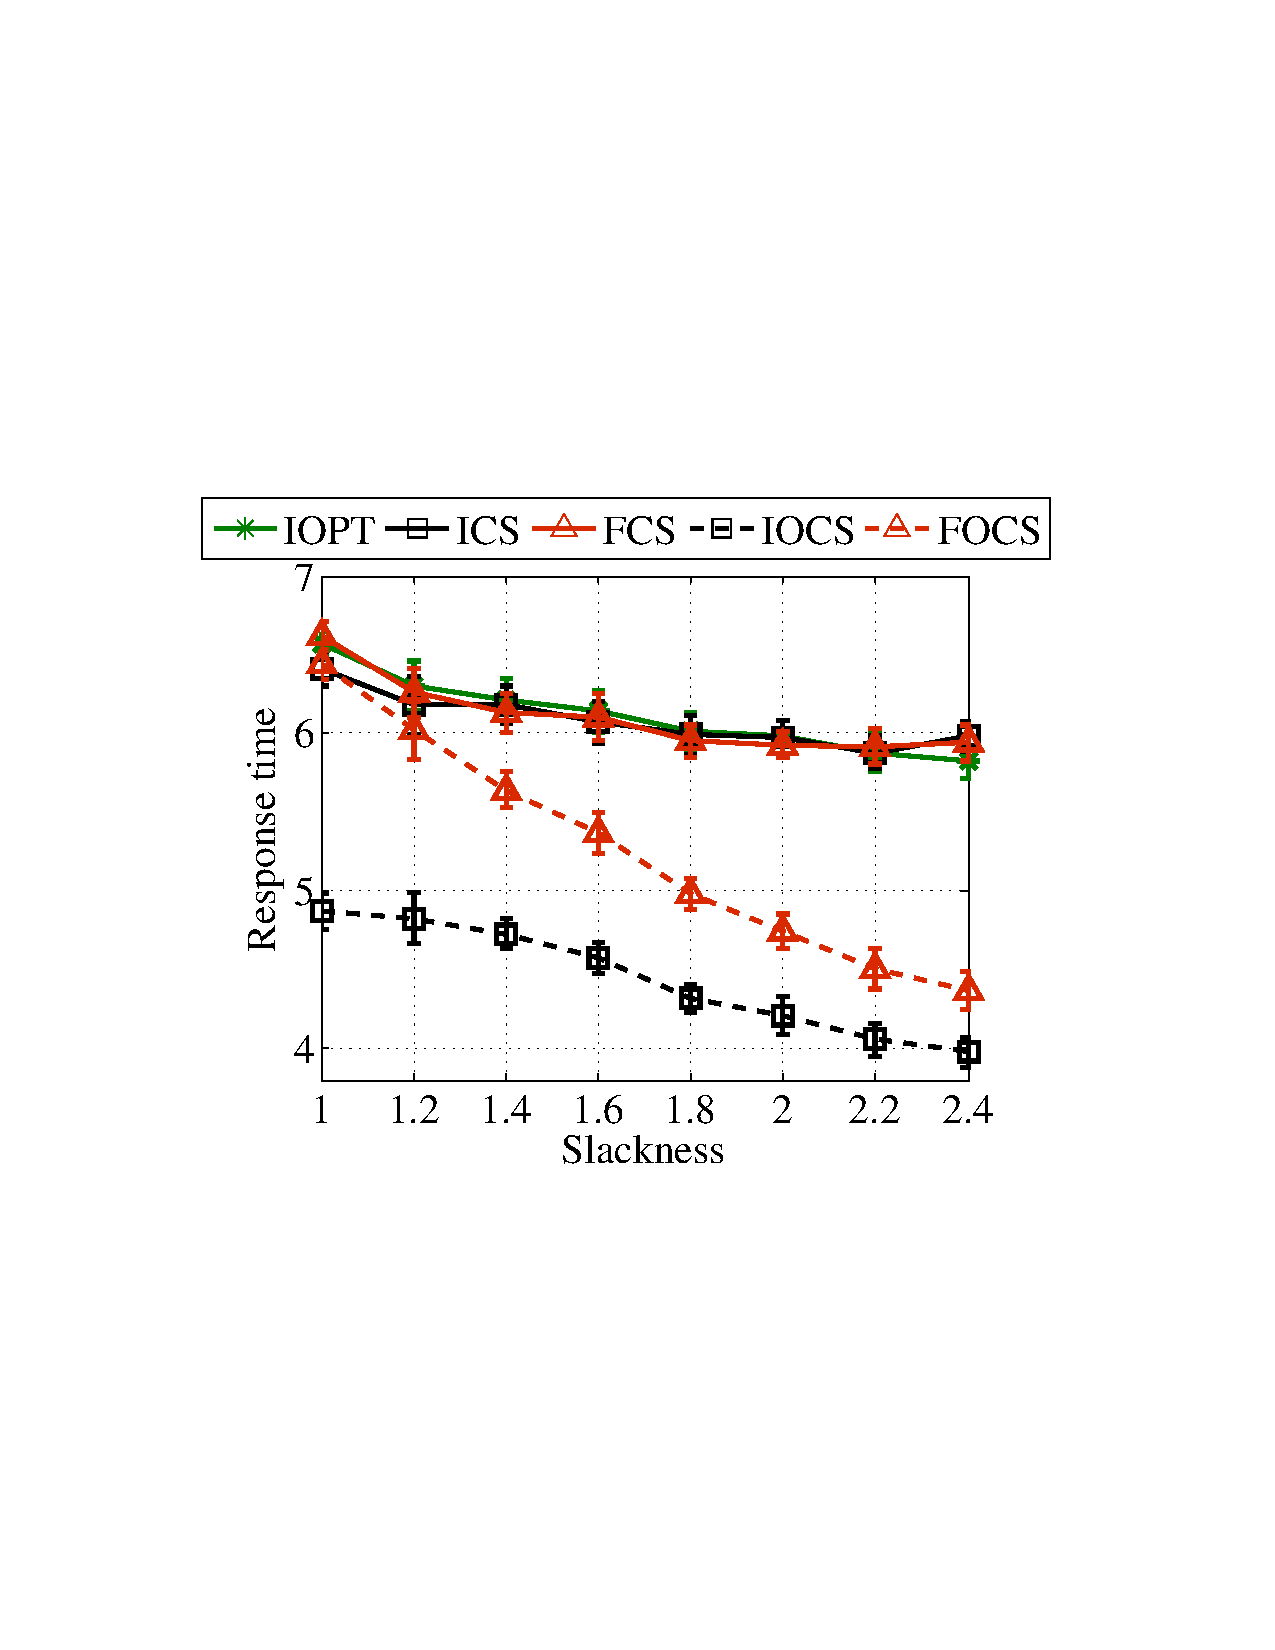
\includegraphics[width=\textwidth]{rt-s-method1.pdf}
%						\caption{Response time (hr))}
%						\label{fig:rt-s-method1}
%					\end{center}
%				\end{subfigure}%  
%\caption{The impact of slackness parameter on total revenue and response time when users react by adjusting their demand.} 
%\label{fig:slackness1}
%\end{figure}
			
%\subsection{The Impact of Slackness Parameter}
%\label{sec:sim:slack}
%This section discusses on the benefits and disadvantages that can be brought by using slackness parameter. To give the charging scheduler more flexibility, a slackness parameter $s\geq 1$ is used and set by the system designer. 
%Recall that charging profile of EV $i$ is feasible if $D_i\leq k_i\frac{d_i-a_i+1}{s}$ holds. Since users have no control on the slackness parameter and the maximum charging rate, they must adjust their demand and availability according to the imposed slackness value. Based on the charging profile feasibility equation, when the slackness value increases users have two choices to react: (i) decrease the demand and depart at the desired deadline or, (ii) extend the deadline and receive the desired demand. In the remaining of this section, we investigate the effects of either case by simulation. To have a clear picture of effects caused by slackness parameter, we generated $100$ initial charging profiles $\langle a_i,d_i,v_i,D_i,k_i\rangle$ for $100$ EVs randomly and uniformly chosen from $10$ different models in Table \ref{tb:models} such that the initial profiles are set up assuming that the CS allows the charging operations to be finished at earliest possible time (i.e., $\frac{D_i}{k_i}$) with $s=1$. For each EV, its demand is randomly chosen from $25\%$ to $100\%$ of its battery capacity and departure in  interval $[a_i+\frac{sD_i}{k_i},T]$, where $a_i+\frac{sD_i}{k_i}$ is the earliest feasible deadline. Then, the EVs are uniformly assigned to $4$ CSs and should choose one of the above strategies to submit a feasible demand according to imposed slackness. 
%\begin{figure}[t]	
%\centering
%							\begin{subfigure}[b]{0.234\textwidth}
%								\begin{center}
%									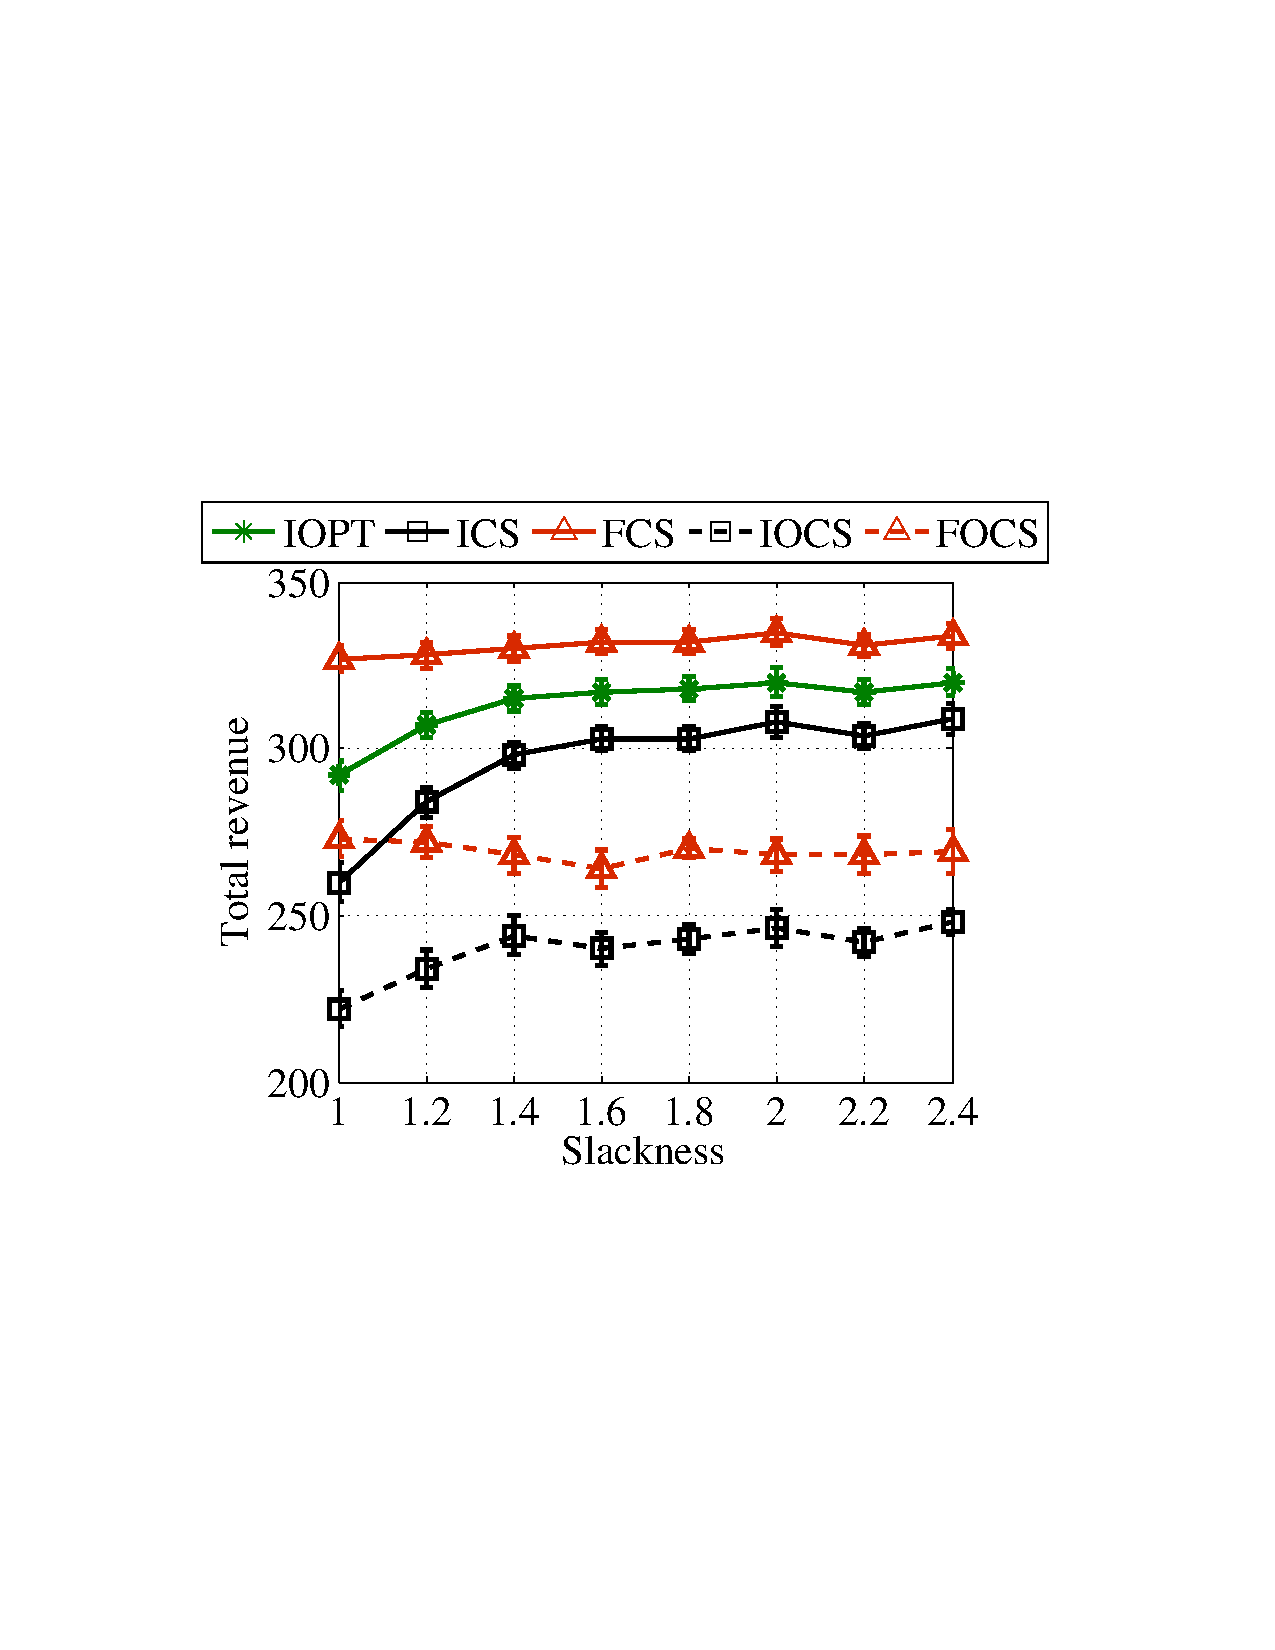
\includegraphics[width=\textwidth]{v-s-method2.pdf}
%									\caption{Total revenue (\$)}
%									\label{fig:v-s-method2}
%								\end{center}
%							\end{subfigure}%
%							\hspace{1mm}
%							\begin{subfigure}[b]{0.236\textwidth}
%								\begin{center}
%									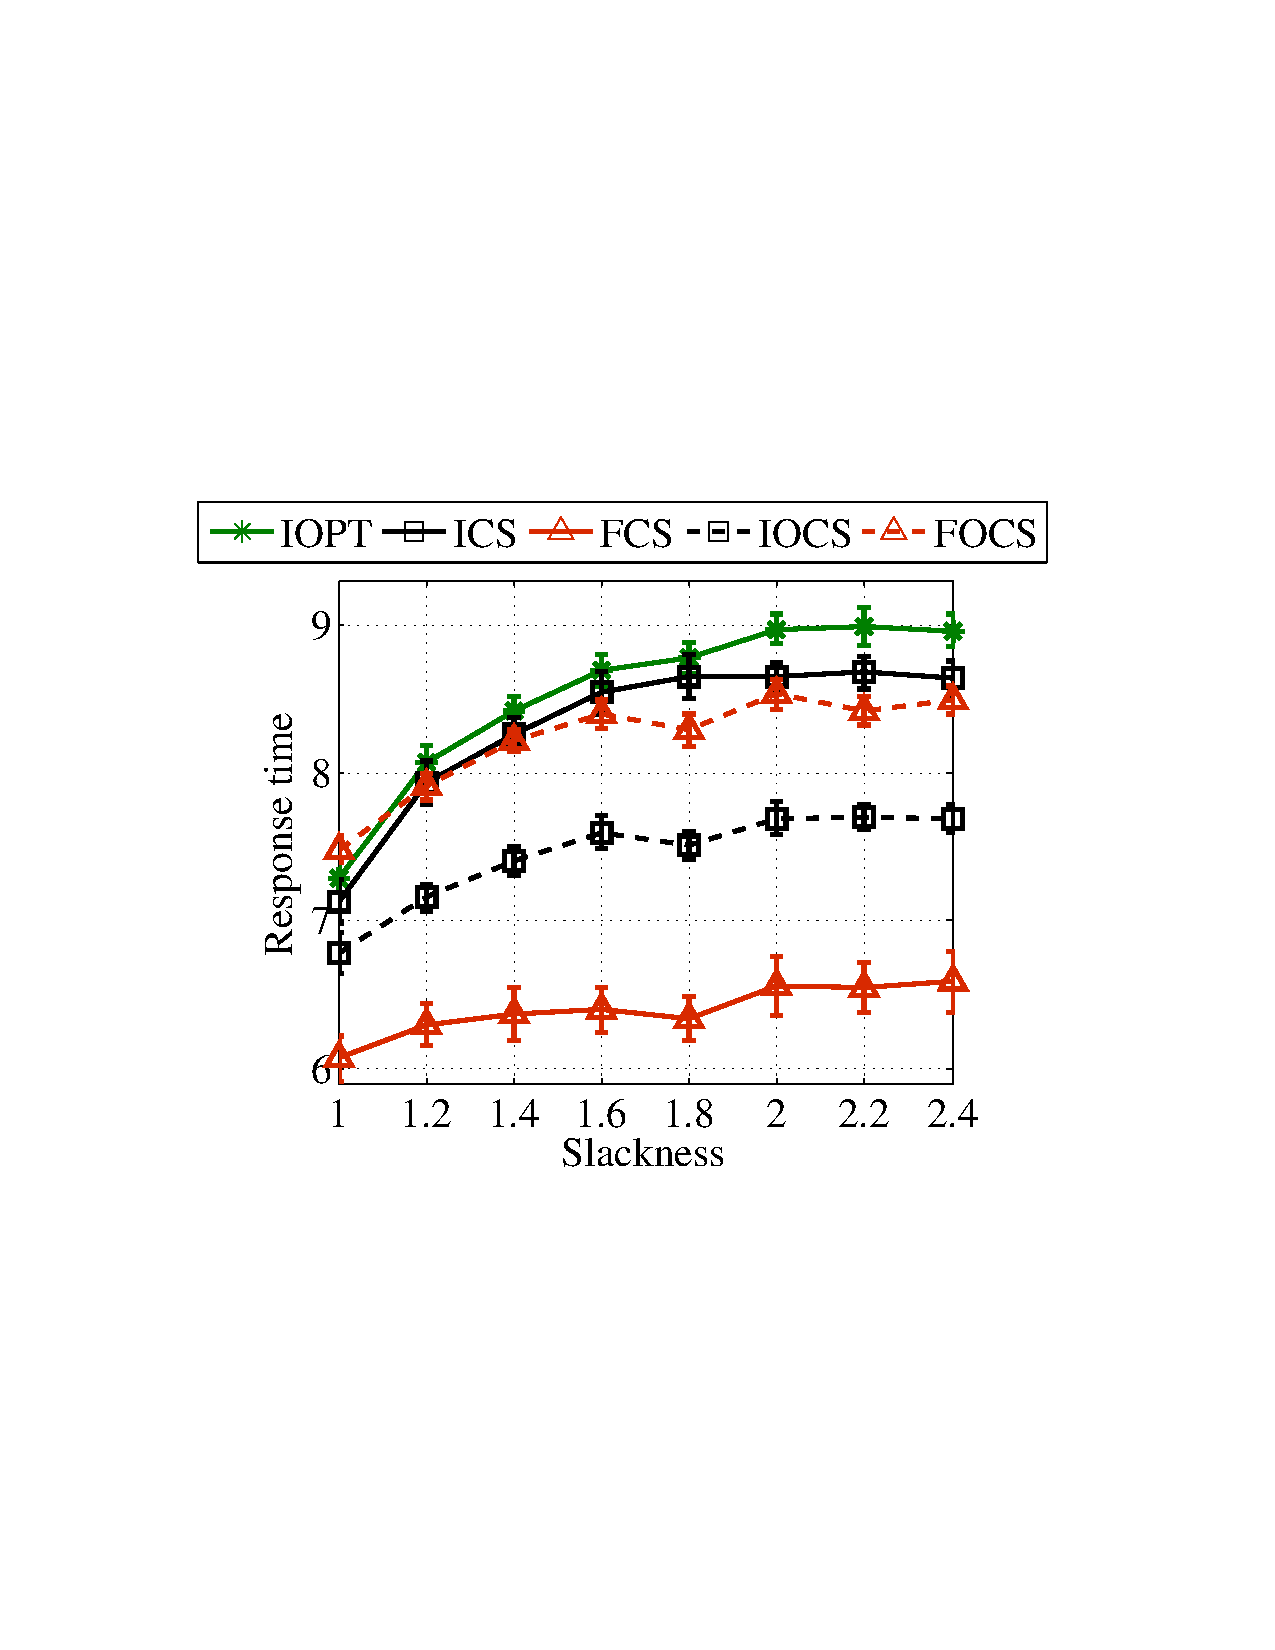
\includegraphics[width=\textwidth]{rt-s-method2.pdf}
%									\caption{Response time (hr)}
%									\label{fig:rt-s-method2}
%								\end{center}
%							\end{subfigure}% 
%							
%\caption{The impact of slackness parameter on total revenue and response time when users react by adjusting their deadline.} 
%\label{fig:slackness2}
%\end{figure}
%			
%\subsubsection{Case I- Adjusting Demands}
%In this case, if the initial charging profile of an EV does not reflect a feasible charging request based on the slackness parameter, the EV owner decreases its demand so it will be able to leave CS at its initial desired deadline. Note that the valuation of EVs decreases proportionally, as well. Fig.~\ref{fig:slackness1} depicts the result under this policy applied by users. As it can be seen in Fig. \ref{fig:v-s-method1} and Fig. \ref{fig:rt-s-method1}, the general trend is that both total revenue and average response time decrease when slackness value increases. This is justifiable based on users reaction. When users decrease their demand, less electricity is sold which results in less revenue. When total demand decreases, charging can be finished in shorter time which decreases response time. Therefore, if users choose the first policy (adjusting their demand), total revenue degrades while response time improves. Notice that for the algorithms working under integral revenue model (i.e., \textsc{iOPT}, \ics and \iocs) the total revenue increases with slackness parameter at first (when $s$ grows from $1$ to $1.4$) but then it decreases when the slackness increases more (for $s>1.4$). 
%In our view, this happens because increasing the slackness in integral revenue model makes it possible to \emph{fully} charge more EVs at the beginning as the demands decrease. However, when the slackness increases more, it results in opposite effect because the valuation of demands decreases along with the demands' size.	
%			\subsubsection{Case II- Adjusting Deadlines}
%			In this case, we assume that users are reluctant to decrease their desired demands. Instead, they can extend their departure. In Fig.~\ref{fig:slackness2} it can be observed that under this behavior of the users, the results are opposite as compared to the previous case (Fig.~\ref{fig:slackness1}). When deadlines are extended without demand decrement, the scheduler has more chance to compliance the demands through improved scheduling flexibility. Consequently, the total revenue increases by increasing slackness value while average response time degrades. 
%%Also observe the behavior of the online algorithms (i.e., \iocs and \focs) where both total revenue and response time decrease after a specific point that is $s=1.8$. When deadlines extend, more EVs have the opportunity of getting charged	
%					
%We can conclude that when total revenue is more important than the response time, the CS should impose small values of slackness for users that apply the policy of the first case and impose higher values of slackness for the users that apply the second policy. The conclusion is reverse for the case that the objective is to have lower response times. 

			%In fact, the slackness parameter controls the maximum demand or earliest deadline that an EV can submit to the system. Remember that demands are in interval $[\textrm{min}\{\frac{d_i-a_i}{sk_i},U_i\},U_i]$ for EV $i$ meaning that the maximum demand that an EV can submit decreases by increasing slackness parameter. A reduction in total demand result in lower charging costs. Therefore, the total revenue decreases with higher values of parameter $s$ as in Fig. \ref{fig:v-s}. 
			%Also, the percentage of EVs that received all of their requested demand increases based on the same fact. The main goal of this simulation is to observe that obtained theoretical result on approximation ratio is confirmed as optimality gap of the SCS algorithm reduces by increasing $s$ in Fig. \ref{fig:v-s}. 
%\vspace{0.1mm}
%\vspace{-4mm}
